\section{РАЗРАБОТКА БАЗЫ ДАННЫХ}
\subsection{Концептуальная модель}

\textbf{Предметная область} - совокупность объектов,
свойства которых и отношения между которыми рассматриваются в рамках некоторого исследования.

\textbf{Модель предметной области} - некоторая система, адекватно имитирующая
структуру и функционирование исследуемой предметной области.

\textbf{Концептуальная модель} - это структура моделируемой предметной области,
свойств её элементов и причинно-следственных связей, присущих системе и
существенных для достижения цели моделирования.
В рамках этапа концептуального моделирования выделяются основные смысловые единицы (сущности)
предметной области, определяются и описываются связи между ними.

Концептуальная модель ориентирована на потенциальных пользователей базы данных,
так как представляет предметную область на их уровне понимания.
Этот уровень называется системно-независимым или предметно-ориентированным.

Основные символы модели данных в ARIS Express 2.4i \cite{ArisExpress} 
изображены на рисунке~\ref{fig:ArisDataModel}.

\begin{figure}[!h]
    \centering

    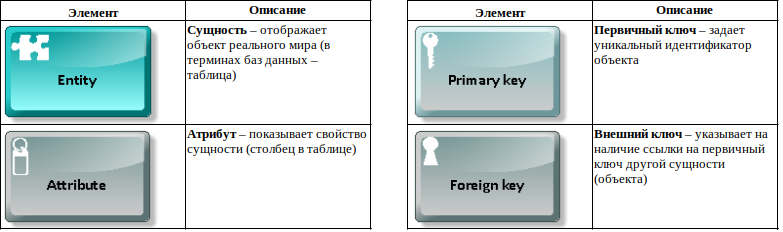
\includegraphics[width=18cm]
    {assets/ARIS/DataModel/Elements/ArisDataModel.png}

    \caption{Основные символы модели данных (ARIS Express 2.4i Data Model)}

    \label{fig:ArisDataModel}
\end{figure}

Модель данных позволяет взглянуть на данные и отношения между ними.
Виды отношений между объектами (1:1, 1:01, 1:0n, 1:1n, 1:n) задаются с помощью атрибутов связей.
Виды связей сущностей в ARIS Express 2.4i \cite{ArisExpress} нотации <<Data Model>> изображены на рисунке~\ref{fig:ArisDataModelRelations}.

\begin{figure}[!h]
    \centering

    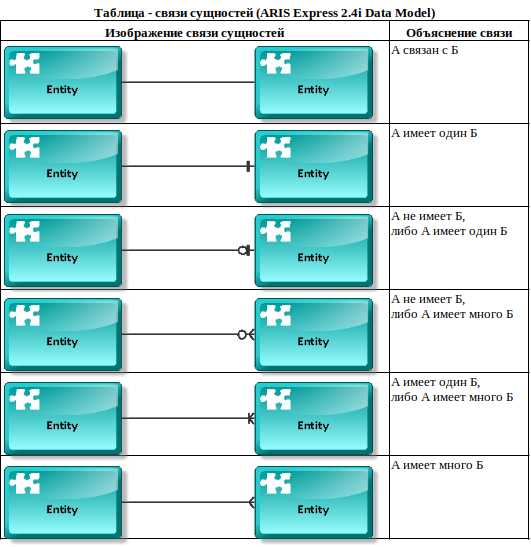
\includegraphics[width=17cm]
    {assets/ARIS/DataModel/Relations/ArisDataModelRelations.png}

    \caption{Связи сущностей}

    \label{fig:ArisDataModelRelations}
\end{figure}

\subsubsection*{Локальная концептуальная модель для процедуры <<Создание инвентаризационной комиссии>>}

ЛКМ (локальная концептуальная модель)
для процедуры <<Создание инвентаризационной комиссии>>
(спроектирована в ARIS Express 2.4 \cite{ArisExpress}, используя нотацию <<Data Model>>)
соответствует функциональному дереву
и изображена на рисунке~\ref{fig:DE_DOC_OrderCreationInventoryCommission}.

\begin{figure}[!h]
    \centering

    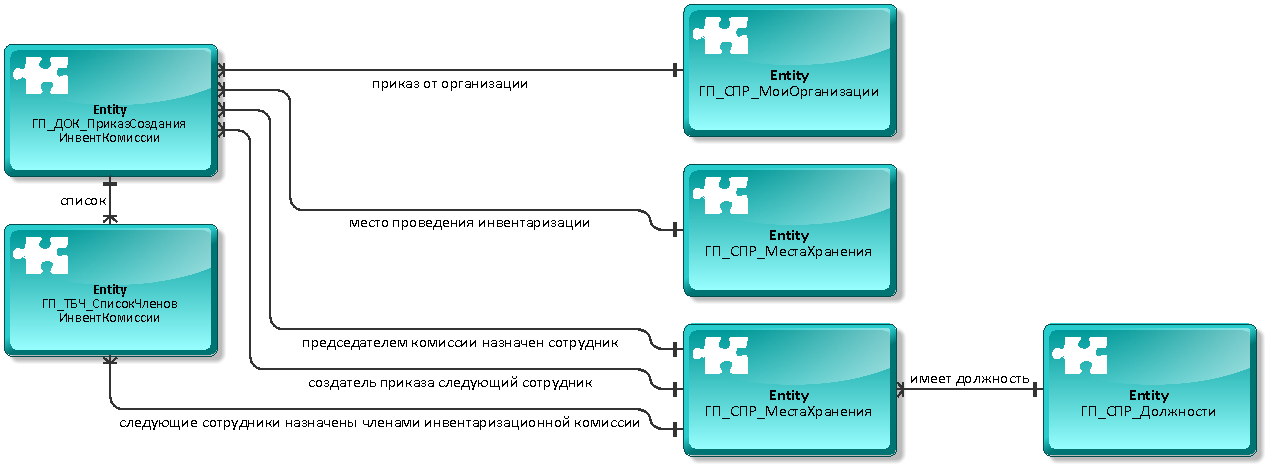
\includegraphics[width=18cm]
    {assets/ARIS/DataModel/ConceptualModels/ГП_ДОК_ПриказСозданияИнвентКомиссии.png}

    \caption{Локальная концептуальная модель для процедуры <<Создание инвентаризационной комиссии>>}

    \label{fig:DE_DOC_OrderCreationInventoryCommission}
\end{figure}

\subsubsection*{Локальная концептуальная модель для процедуры <<Проведение инвентаризации>>}

ЛКМ (локальная концептуальная модель)
для процедуры <<Проведение инвентаризации>>
(спроектирована в ARIS Express 2.4 \cite{ArisExpress}, используя нотацию <<Data Model>>)
соответствует функциональному дереву
и изображена на рисунке~\ref{fig:DE_DOC_InventoryList}.

\begin{figure}[!h]
    \centering

    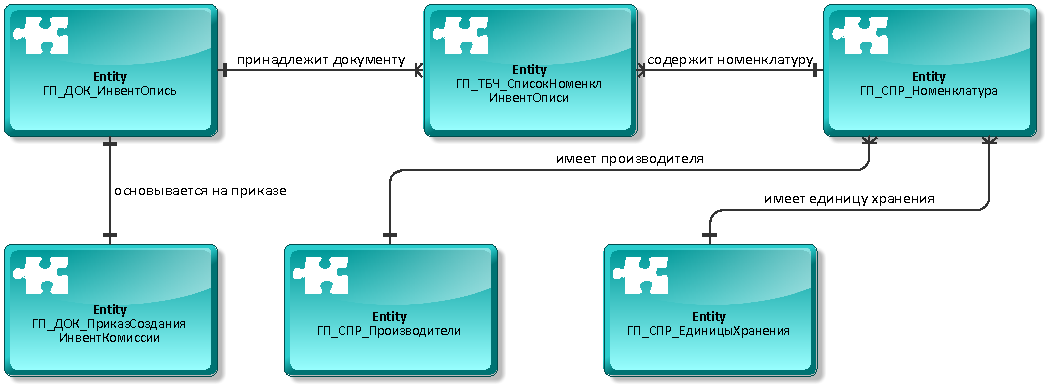
\includegraphics[width=18cm]
    {assets/ARIS/DataModel/ConceptualModels/ГП_ДОК_ИнвентОпись.png}

    \caption{Локальная концептуальная модель для процедуры <<Создание инвентаризационной комиссии>>}

    \label{fig:DE_DOC_InventoryList}
\end{figure}

\subsubsection*{Общая концептуальная модель}

Концептуальная модель строится из локальных концептуальных моделей.

Концептуальная модель
(спроектированна с использованием ARIS Express 2.4 \cite{ArisExpress} нотацией <<Data Model>>)
состоит из локальных концептуальных моделей и
изображена на рисунке~\ref{fig:GeneralConceptualModel}.

\begin{figure}[!h]
    \centering

    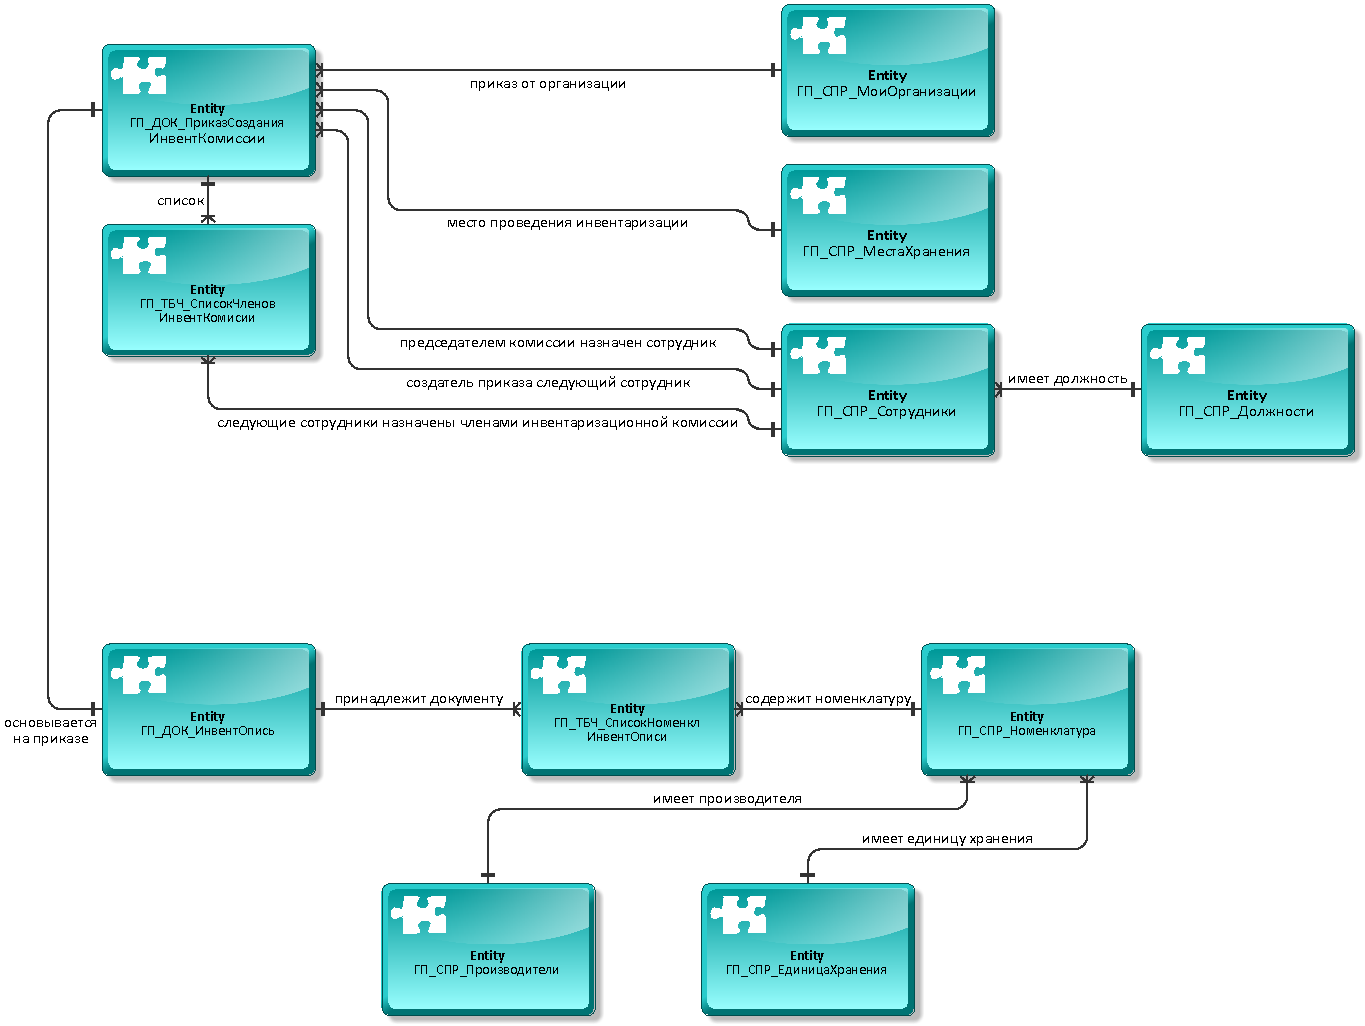
\includegraphics[width=18cm]
    {assets/ARIS/DataModel/GeneralConceptualModel/GeneralConceptualModel.png}

    \caption{Общая концептуальная модель}

    \label{fig:GeneralConceptualModel}
\end{figure}

\subsection{Логическая модель}

\textbf{Логическая модель} - это модель данных конкретной предметной области,
представленной в виде таблиц и их связей.

Виды связей между таблицами в SQL Power Architect 1.0.7 \cite{SqlPowerArhitect}
изображены на рисунке~\ref{fig:RelationsSqlPowerArchitect}.

\begin{figure}[!h]
    \centering

    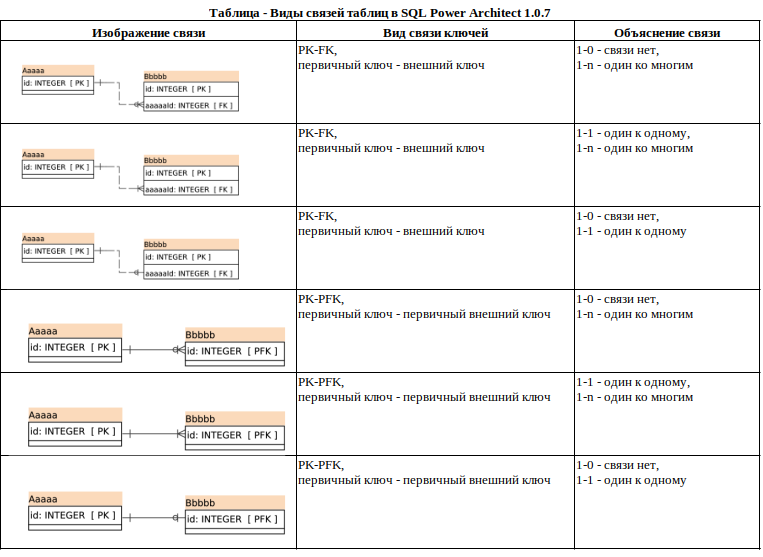
\includegraphics[width=18cm]
    {assets/database/Relations/RelationsSqlPowerArchitect.png}

    \caption{Виды связей таблиц в SQL Power Architect 1.0.7}

    \label{fig:RelationsSqlPowerArchitect}
\end{figure}

\textbf{Физическая модель} - это представление в виде SQL скриптов, которые создают таблицы и связи между таблицами,
которые получаются из логической модели используя генераторы, например, SQL Power Architect.

\textbf{Первая нормальная форма} (1НФ) \cite{habr_1nf_6nf}.
Отношение находится в 1НФ, если все его атрибуты являются простыми,
все используемые домены должны содержать только скалярные значения.
Не должно быть повторений строк в таблице.

\textbf{Вторая нормальная форма} (2НФ) \cite{habr_1nf_6nf}.

Отношение находится во 2НФ, если оно находится в 1НФ и каждый не ключевой атрибут неприводимо зависит от Первичного Ключа (PK).

\textbf{Третья нормальная форма} (3НФ) \cite{habr_1nf_6nf}.

Отношение находится в 3НФ, когда находится во 2НФ и каждый не ключевой атрибут нетранзитивно зависит от первичного ключа.
Второе правило требует выносить все не ключевые поля, содержимое которых может относиться к нескольким записям таблицы в отдельные таблицы.

\textbf{Механизмы целостности} нужны для того, чтобы избежать ситуации не правильного заполнения базы данных.
Для атрибута выбирается тип данных, а у типа данных есть какой-то домен. Например, суть домена <<Код>> состоит в том,
что это целое число (тип INTEGER) и оно больше нуля (CHECK id > 0).
Также могут возникнуть ситуации, когда в базе данных не нужны, либо нужны те или иные атрибуты.
Для этого атрибуту можно присвоить NOT NULL, то есть атрибут важен для заполнения и не может быть пустым.
Когда атрибут не задан, то в базе данных он имеет значение NULL.
В базе данных можно предусмотреть DEFAULT-значения, например, если мы не задали дату,
то у нас отработает процедура NOW(), которая поставит текущую дату.

% = = = = = = = = = = = = = = = = = = = = = = = = = = = = = = = =

\subsubsection*{Таблица для оперативного документа <<Приказ о создании инвентаризационной комиссии>>}

Таблица с механизмами целостности изображена на рисунке~\ref{fig:Logic_DE_DOC_OrderCreationInventoryCommission}.

\begin{figure}[!h]
    \centering

    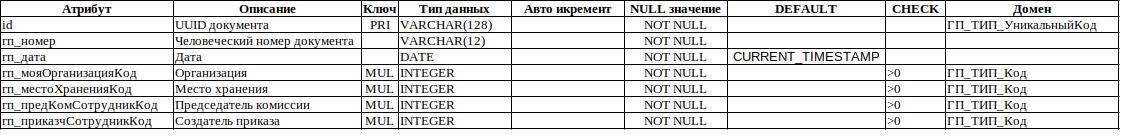
\includegraphics[width=18cm]
    {assets/database/Types/ГП_ДОК_ПриказСозданияИнвентКомиссии.png}

    \caption{Таблица ГП\_ДОК\_ПриказСозданияИнвентКомиссии}

    \label{fig:Logic_DE_DOC_OrderCreationInventoryCommission}
\end{figure}

% = = = = = = = = = = = = = = = = = = = = = = = = = = = = = = = =

\subsubsection*{Таблица справочного документа <<Мои организации>>}

Таблица с механизмами целостности изображена на рисунке~\ref{fig:Logic_DE_CTL_MyOrganization}.

\begin{figure}[!h]
    \centering

    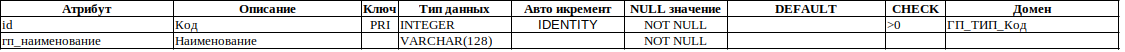
\includegraphics[width=18cm]
    {assets/database/Types/ГП_СПР_МоиОрганизации.png}

    \caption{Таблица ГП\_СПР\_МоиОрганизации}

    \label{fig:Logic_DE_CTL_MyOrganization}
\end{figure}

% = = = = = = = = = = = = = = = = = = = = = = = = = = = = = = = =

\subsubsection*{Таблица справочного документа <<Места хранения>>}

Таблица с механизмами целостности изображена на рисунке~\ref{fig:Logic_DE_CTL_StorageLocations}.

\begin{figure}[!h]
    \centering

    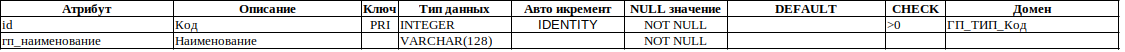
\includegraphics[width=18cm]
    {assets/database/Types/ГП_СПР_МестаХранения.png}

    \caption{Таблица ГП\_СПР\_МестаХранения}

    \label{fig:Logic_DE_CTL_StorageLocations}
\end{figure}

% = = = = = = = = = = = = = = = = = = = = = = = = = = = = = = = =

\subsubsection*{Табличная часть <<Список членов инвентаризационной комиссии>>}

Таблица с механизмами целостности изображена на рисунке~\ref{fig:Logic_DE_TAB_ListInventoryCommission}.

\begin{figure}[!h]
    \centering

    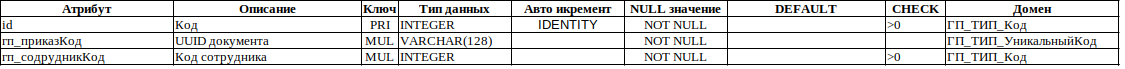
\includegraphics[width=18cm]
    {assets/database/Types/ГП_ТБЧ_СписокЧленовИнвентКомиссии.png}

    \caption{Таблица ГП\_ТБЧ\_СписокЧленовИнвентКомиссии}

    \label{fig:Logic_DE_TAB_ListInventoryCommission}
\end{figure}

% = = = = = = = = = = = = = = = = = = = = = = = = = = = = = = = =

\subsubsection*{Таблица справочного документа <<Сотрудники>>}

Таблица с механизмами целостности изображена на рисунке~\ref{fig:Logic_DE_CTL_Employees}.

\begin{figure}[!h]
    \centering

    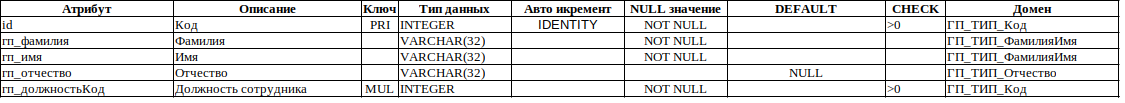
\includegraphics[width=18cm]
    {assets/database/Types/ГП_СПР_Сотрудники.png}

    \caption{Таблица ГП\_СПР\_Сотрудники}

    \label{fig:Logic_DE_CTL_Employees}
\end{figure}

% = = = = = = = = = = = = = = = = = = = = = = = = = = = = = = = =

\subsubsection*{Таблица справочного документа <<Должности>>}

Таблица с механизмами целостности изображена на рисунке~\ref{fig:Logic_DE_CTL_Positions}.

\begin{figure}[!h]
    \centering

    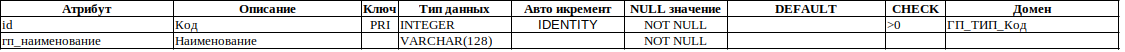
\includegraphics[width=18cm]
    {assets/database/Types/ГП_СПР_Должности.png}

    \caption{Таблица ГП\_СПР\_Должности}

    \label{fig:Logic_DE_CTL_Positions}
\end{figure}

% = = = = = = = = = = = = = = = = = = = = = = = = = = = = = = = =

\subsubsection*{Таблица оперативного документа <<Инвентаризационная опись>>}

Таблица с механизмами целостности изображена на рисунке~\ref{fig:Logic_DE_DOC_InventoryList}.

\begin{figure}[!h]
    \centering

    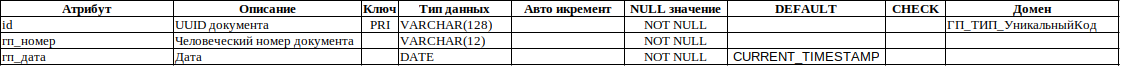
\includegraphics[width=18cm]
    {assets/database/Types/ГП_ДОК_ИнветОпись.png}

    \caption{Таблица ГП\_ДОК\_ИнветОпись}

    \label{fig:Logic_DE_DOC_InventoryList}
\end{figure}

% = = = = = = = = = = = = = = = = = = = = = = = = = = = = = = = =

\subsubsection*{Табличная часть <<Список номенклатуры инвентаризационной описи>>}

Таблица с механизмами целостности изображена на рисунке~\ref{fig:Logic_DE_TAB_NomenclatureInventList}.

\begin{figure}[!h]
    \centering

    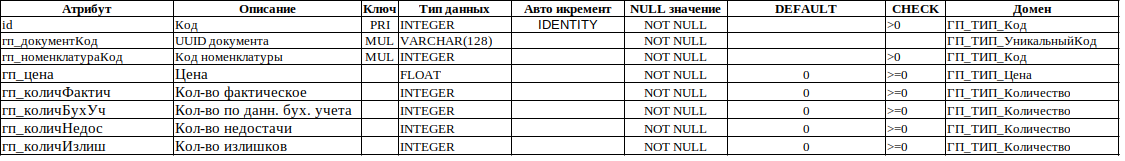
\includegraphics[width=18cm]
    {assets/database/Types/ГП_ТБЧ_СписокНоменклИнвентОписи.png}

    \caption{Таблица ГП\_ТБЧ\_СписокНоменклИнвентОписи}

    \label{fig:Logic_DE_TAB_NomenclatureInventList}
\end{figure}

% = = = = = = = = = = = = = = = = = = = = = = = = = = = = = = = =

\subsubsection*{Таблица справочного документа <<Номенклатура>>}

Таблица с механизмами целостности изображена на рисунке~\ref{fig:Logic_DE_CTL_Nomenclatures}.

\begin{figure}[!h]
    \centering

    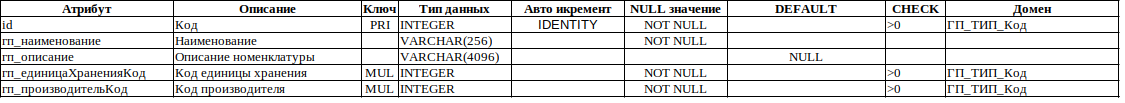
\includegraphics[width=18cm]
    {assets/database/Types/ГП_СПР_Номенклатура.png}

    \caption{Таблица ГП\_СПР\_Номенклатура}

    \label{fig:Logic_DE_CTL_Nomenclatures}
\end{figure}

% = = = = = = = = = = = = = = = = = = = = = = = = = = = = = = = =

\subsubsection*{Механизмы целостности для справочника <<Единицы хранения>>}

Таблица с механизмами целостности изображена на рисунке~\ref{fig:Logic_DE_CTL_StorageUnits}.

\begin{figure}[!h]
    \centering

    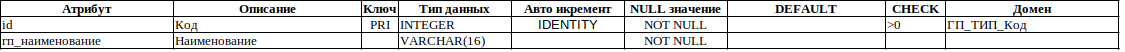
\includegraphics[width=18cm]
    {assets/database/Types/ГП_СПР_ЕдиницыХранения.png}

    \caption{Таблица ГП\_СПР\_ЕдиницыХранения}

    \label{fig:Logic_DE_CTL_StorageUnits}
\end{figure}

% = = = = = = = = = = = = = = = = = = = = = = = = = = = = = = = =

\subsubsection*{Механизмы целостности для справочника <<Производители>>}

Таблица с механизмами целостности изображена на рисунке~\ref{fig:Logic_DE_CTL_Producers}.

\begin{figure}[!h]
    \centering

    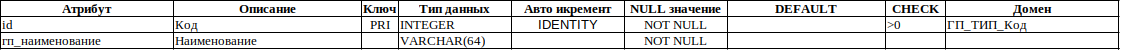
\includegraphics[width=18cm]
    {assets/database/Types/ГП_СПР_Производители.png}

    \caption{Таблица ГП\_СПР\_Производители}

    \label{fig:Logic_DE_CTL_Producers}
\end{figure}

% = = = = = = = = = = = = = = = = = = = = = = = = = = = = = = = =

\subsubsection*{Проектирование логической модели}

Логическая модель доведенная до третьей нормальной формы,
спроектированная в SQL Power Architect 1.0.7 \cite{SqlPowerArhitect},
изображена на рисунке~\ref{fig:logic_model}.

\begin{figure}[!h]
    \centering

    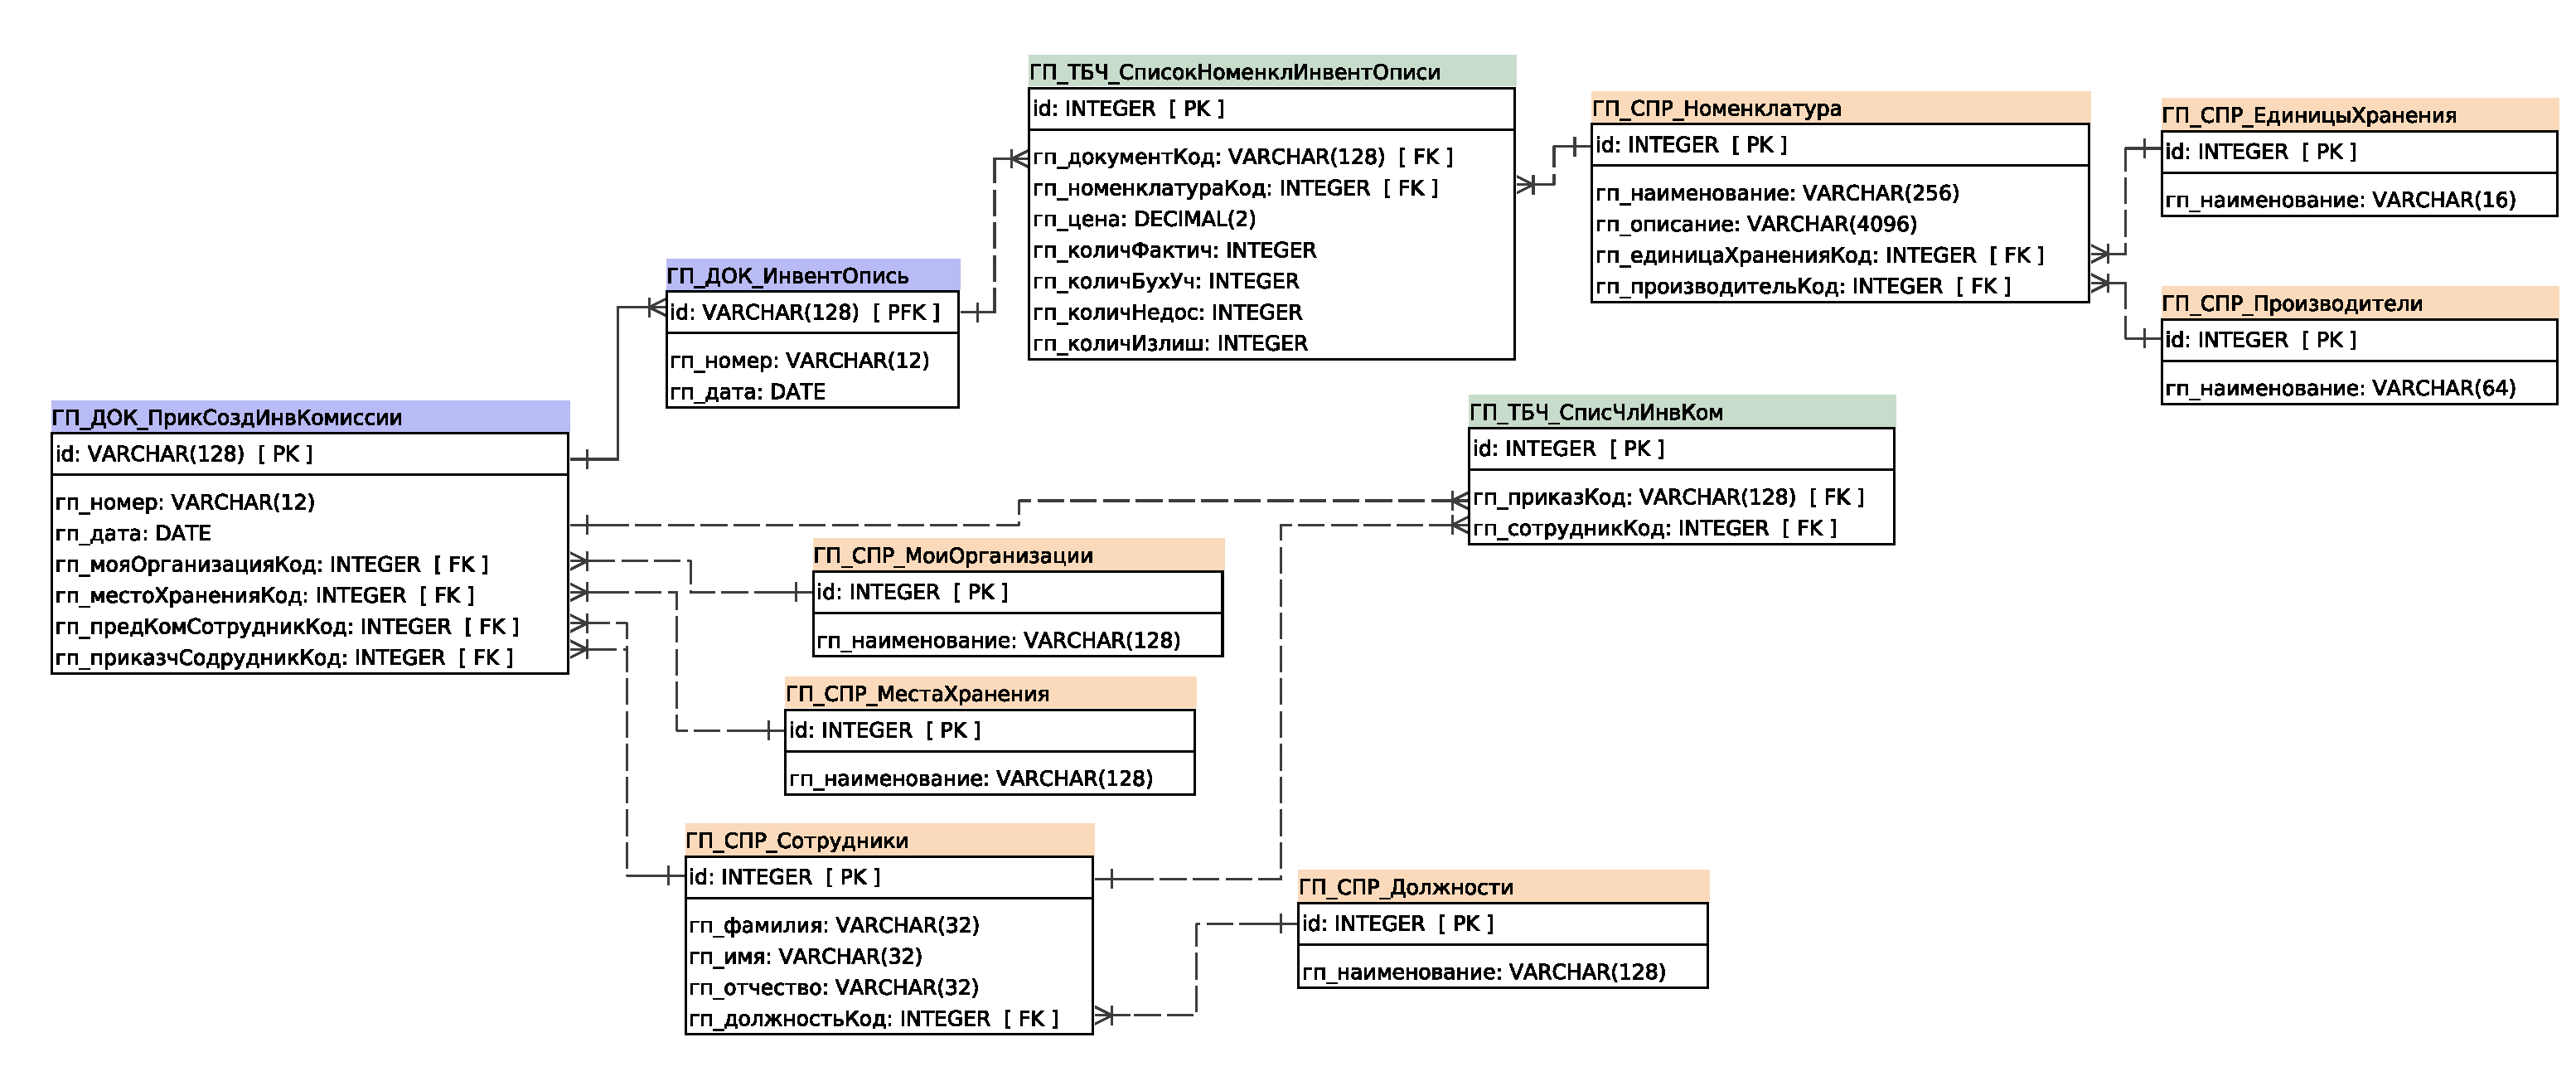
\includegraphics[width=18cm]
    {assets/database/SqlPowerArchitect/logic_model.pdf}

    \caption{Логическая модель}

    \label{fig:logic_model}
\end{figure}

\subsection{Физическая модель}

\textbf{Физическая модель} - это представление в виде SQL скриптов, которые создают таблицы и связи между таблицами,
которые получаются из логической модели используя генераторы, например, SQL Power Architect.

% Docker - программа, которая устанавливает в изолированном контейнере программу.
% Например, можно установить в контейнере MySQL. Для этого нужен файл <<docker-compose.mysql.yml>> и файл с паролями <<.env>>.

% \begin{lstlisting}[language=bash, name={Установка Docker}]
% sudo apt update
% sudo apt install docker
% sudo apt install docker-compose
% \end{lstlisting}

% \begin{lstlisting}[name={docker-compose.mysql.yml}]
% version: "3"

% services:
%     db:
%     image: mysql:8.0
%     ports:
%         - 3307:3306
%     command: --default-authentication-plugin=mysql_native_password
%     environment:
%         MYSQL_DATABASE: ${MYSQL_DATABASE}
%         MYSQL_USER: ${MYSQL_USER}
%         MYSQL_PASSWORD: ${MYSQL_PASSWORD}
%         MYSQL_ROOT_PASSWORD: ${MYSQL_ROOT_PASSWORD}
%     volumes:
%         - ./docker/mysql/initdb.d:/docker-entrypoint-initdb.d
%         - ./docker/mysql/etc/mysql/conf.d:/etc/mysql/conf.d
%         - ./docker/mysql/var/lib/mysql:/var/lib/mysql
%     phpmyadmin:
%     image: phpmyadmin/phpmyadmin
%     container_name: phpmyadmin
%     links: 
%         - db:db
%     ports:
%         - 3080:80
%     environment:
%         MYSQL_USER: ${MYSQL_USER}
%         MYSQL_PASSWORD: ${MYSQL_PASSWORD}
%         MYSQL_ROOT_PASSWORD: ${MYSQL_ROOT_PASSWORD} 
% \end{lstlisting}

% \begin{lstlisting}[name={Файл с секретами .env}]
% MYSQL_DATABASE=database
% MYSQL_USER=super_secret_user
% MYSQL_PASSWORD=super_secret_password
% MYSQL_ROOT_PASSWORD=super_secret_root_password
% \end{lstlisting}

% \begin{lstlisting}[language=bash, name={Запуск базы данных}]
% docker-compose -f database/docker-compose.mysql.yml up
% \end{lstlisting}

% \begin{lstlisting}[language=bash, name={Установка консольного клиента}]
% sudo apt update
% sudo apt install mysql-client
% \end{lstlisting}

% \begin{lstlisting}[language=bash, name={Подключение через консольный клиент}]
% mysql -h localhost -P 3307 --protocol=tcp -u super_secret_user -D database -p'super_secret_password'
% source ./logic_model_create.sql # выполняем SQL скрипт
% exit
% \end{lstlisting}

% \begin{lstlisting}[name=Установка MySQL на Linux Ubuntu 22.04]
% sudo apt update
% sudo apt install mysql-server
% sudo systemctl start mysql.service

% sudo mysql
% ALTER USER 'root'@'localhost' IDENTIFIED WITH mysql_native_password BY '((super#SECRET#password#123))';
% exit
% \end{lstlisting}

% \begin{lstlisting}[name=Установка пароля root для MySQL]
% sudo mysql
% ALTER USER 'root'@'localhost' IDENTIFIED WITH mysql_native_password BY '((super#SECRET#password#123))';
% exit

% sudo mysql -u root -p # вводим пароль ((super#SECRET#password#123))
% ALTER USER 'root'@'localhost' IDENTIFIED WITH auth_socket;
% \end{lstlisting}

% \begin{lstlisting}[name=Создание базы данных]
% sudo mysql -u root -p # вводим пароль ((super#SECRET#password#123))
% CREATE DATABASE st190333_7sem_coursework;
% exit
% \end{lstlisting}

% \begin{lstlisting}[name=Создание пользователя]
% sudo mysql -u root -p # вводим пароль ((super#SECRET#password#123))
% CREATE USER 'st190333_'@'localhost' IDENTIFIED WITH mysql_native_password BY '((SUPER#secret#password#123))';
% exit
% \end{lstlisting}

% \begin{lstlisting}[name=Создание пользователя]
% sudo snap install mysql-workbench-community
% \end{lstlisting}

Физическую модель получим из логической модели нажав кнопку <<Forward Engineer SQL Script>>
в SQL Power Arhitect 1.0.7 \cite{SqlPowerArhitect}.
Так как SQL Power Architect не имеет возможности генерировать CHECK'и,
то пропишем их в скрипте сами.

Для удобства проверки БД использовались скрипт удаления БД DROP DATABASE \cite{MssqlDropDatabase} (см. листинг~\ref{lst:DropDatabase})
и скрипт создания БД CREATE DATABASE \cite{MssqlCreateDatabase} (см. листинг~\ref{lst:CreateDatabase}).

\begin{lstlisting}[caption={Удаление базы данных\label{lst:DropDatabase}}]
DROP DATABASE [ IF EXISTS ] <имяБД>
[;]
\end{lstlisting}

\begin{lstlisting}[caption={Создание базы данных\label{lst:CreateDatabase}}]
CREATE DATABASE <имяБД>
[;]
\end{lstlisting}

Таблицы создаются через команду CREATE TABLE \cite{MssqlCreateTable} (см. листинг~\ref{lst:CreateTable}).

\begin{lstlisting}[caption={Создание таблицы\label{lst:CreateTable}}]
CREATE TABLE { <имяБД>.<имяСхемы>.<имяТаблицы> | <имяСхемы>.<имяТаблицы> | <имяТаблицы> }
(
    <атрибут> <тип> [NOT NULL] [DEFAULT <значение>] [CHECK(<атрибут> <условие>)]
    [ , <атрибут> <тип> [NOT NULL] [DEFAULT <значение>] [CHECK(<атрибут> <условие>)]]
)
[ ; ]
\end{lstlisting}

Таблицы связываем по полям, используя ALTER TABLE \cite{MssqlAlterTable} (см. листинг~\ref{lst:AlterTable}), чтобы исключить случай удаления данных, которые зависят от нашей таблицы.

\begin{lstlisting}[caption={Связываем таблицы по полям\label{lst:AlterTable}}]
ALTER TABLE <имяТаблицы> ADD CONSTRAINT <имяВнешнегоКлюча>__fk
FOREIGN KEY (<имяАтрибутаТаблицы>)
REFERENCES <имяВторойТаблицы> (<имяАтрибутаТаблицы>)
ON DELETE NO ACTION
ON UPDATE NO ACTION
[;]
\end{lstlisting}

В СУБД Microsoft SQL Server есть возможность создавать свой тип данных через команду CREATE TYPE \cite{MssqlCreateType} (см. листинг~\ref{lst:CreateType}).

\begin{lstlisting}[caption={Связываем таблицы по полям\label{lst:CreateType}}]
CREATE TYPE
    FROM <тип> [NOT NULL]
[;]
\end{lstlisting}

SQL-скрипт генерируется в SQL Power Architect \cite{SqlPowerArhitect} при проектировании логической модели.
Это скрипт можно подредактировать добавив типы данных (CREATE TYPE) и добавив ограничения (CHECK).
Готовый скрипт изображен на листинге~\ref{lst:sqlScript}.

\lstinputlisting[language=sql, caption={Скрипт создания БД и таблиц в ней\label{lst:sqlScript}}]
{sql/0.sql}

\newpage
